\documentclass[fontsize=10pt]{article}
\usepackage[margin=0.70in]{geometry}
\usepackage{lipsum,mwe,abstract}
\usepackage[T1]{fontenc} 
\usepackage[english]{babel} 

\usepackage{fancyhdr} % Custom headers and footers
%\pagestyle{fancyplain} % Makes all pages in the document conform to the custom headers and footers
%\fancyhead{} 
\fancyfoot[C]{\thepage} % Page numbering for right footer
\usepackage{lipsum}
\setlength\parindent{0pt} 

\usepackage{amsmath,amsfonts,amsthm} % Math packages
\usepackage{wrapfig}
\usepackage{graphicx}
\usepackage{float}
\usepackage{subcaption}
\usepackage{adjustbox}
\usepackage{comment}
\usepackage{enumitem}
\usepackage{cuted}
\usepackage{pgfplots}
\pgfplotsset{compat=1.9}

\usepackage{sectsty} % Allows customizing section commands
\usepackage{kotex}

\allsectionsfont{\normalfont \normalsize \scshape} % Section names in small caps and normal fonts

\renewenvironment{abstract} % Change how the abstract look to remove margins
 {\small
  \begin{center}
  \bfseries \abstractname\vspace{-.5em}\vspace{0pt}
  \end{center}
  \list{}{%
    \setlength{\leftmargin}{0mm}
    \setlength{\rightmargin}{\leftmargin}%
  }
  \item\relax}
 {\endlist}
 
\makeatletter
\renewcommand{\maketitle}{\bgroup\setlength{\parindent}{0pt} % Change how the title looks like
\begin{flushleft}
  \textbf{\@title}
  \@author \\ 
  \@date
\end{flushleft}\egroup
}
\makeatother

%% ------------------------------------------------------------------- 

\title{
\Large Feature engineering for efficiently detecting Modbus/TCP anomaly \\
[10pt] 
}
\date{\today}
\author{Jinseok Park, Geonwoo Lee}

\begin{document}

\maketitle

% --------------- ABSTRACT
\begin{abstract}
As the number of smart factory increases, the factory's network changes from a closed network to an open concept, increasing the need to respond to attacks that can come through external networks. Accordingly, in this study, we investigate which learning base detection model and which feature set can effectively detect anomaly quickly and accurately on Modbus/TCP networks. Among the SVM, DT, Random Forest, Kmeans, DNN, and Autoencoder models, DT has the fastest throughput and stable accuracy compared to other models, while DNN models and Autoencoder models have high accuracy and acceptable process speed.
\end{abstract}

\rule{\linewidth}{0.5pt}

% --------------- MAIN CONTENT

\section{Introduction}
Recently, in the advent of the Fourth Industrial Revolution, smart factories with strong connection-oriented characteristics have emerged, escaping from the closed network concept. Unlike a closed network base factory environment, the Industrial Control System(ICS) of a smart factory tends to be connected to the external internet, and it means that system is exposed to several security threats that have not been considered before. Therefore, there is a need to come up with countermeasures against attacks coming from external networks.


In this paper, we studied which detection model and which feature extraction method would be most efficient to detect network anomalies, such as DDoS, during network attacks. We limit the target to Modbus/TCP for network protocol and only considered Machine Learning-based detection models because the Rule-based model needs manual rule generation and management taking more cost than learning-based model in the long term.



About learning-based anomaly detection models, we focused on these two factors.
\begin{itemize}
    \item [.] feature extraction : which feature best represent abnormal behavior?
    \item [.] detection model: which model is most accurate and efficient(fast)?
\end{itemize}
We conducted intensive research on the two topics and conducted them between May and early June this year.


\section{Approaches}
\subsection{Dataset}
To train anomaly detection models, dataset and their quality are very important. Unfortunately, we could not get hardware to simulate the CPS environment, so we should continue our research by using the existing dataset. The dataset used in the study, CYBER-SECURITY MODBUS ICS DATASET \cite{pjff-1a03-19}, is a dataset that exists in IEEE dataport. It simulated the following small industrial networks and then generated several anomalies, such as DDoS/MITM.


We created a dataset by extracting features from each packet of the original dataset and labeling each of them by attack type. The composition of the dataset that we created is as follows.
\begin{center}
    \begin{tabular}{|c|c|}
        \multicolumn{2}{c}{\textbf{\large Datasets class type}} \\ \hline
        \textbf{Type}                & \textbf{number(packet)}         \\ \hline
        Normal                       & 1208554(during attack) + 521686 \\ \hline
        MITM                         & 47083                           \\ \hline
        Modbus Query Flooding        & 893233                          \\ \hline
        Ping Flooding                & 754232                          \\ \hline
        TCP SYN Flooding             & 698758                          \\ \hline
        Total                        & 4123546                         \\ \hline
    \end{tabular}
\end{center}
\begin{center}
    \begin{tabular}{|c|c|}
        \multicolumn{2}{c}{\textbf{\large Portion of Train and Test set}} \\ \hline
        \textbf{Usage}              & \textbf{number(packet)}         \\ \hline
        Train                       & 2474127 (60\%)                      \\ \hline
        Test                        & 1649419 (40\%)                     \\ \hline
    \end{tabular}
\end{center}

We limited the number of feature data from attack packets to balance normal and attack packets feature data in the datasets, and used 60\% of them for training, and used the rest 40\% for testing. We did feature engineering by using this dataset, by limiting some features in training and testing anomaly detection models.


\subsection{Overview}
To simultaneously evaluate the extracted feature set and the performance of the detection model, we construct the framework as follows.
\begin{figure}[!htbp]
\centering
   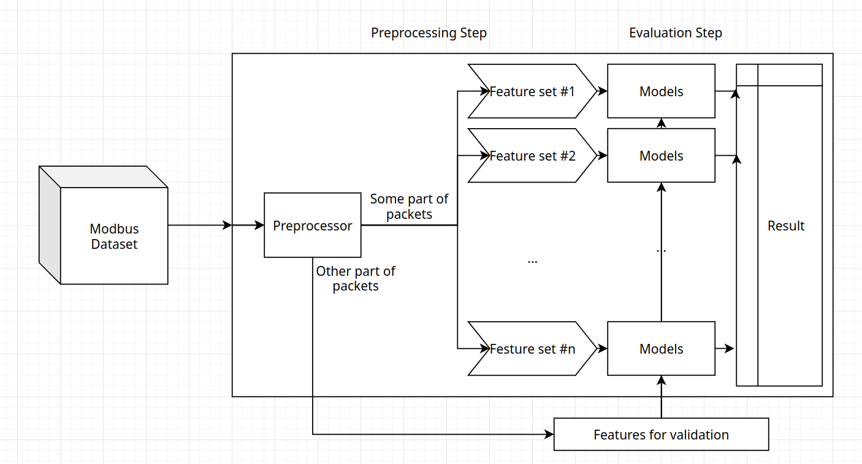
\includegraphics[width=14cm]{overview}
   \hfil
\caption{framework overview}
\label{overview}
\end{figure}


The framework is largely divided into pre-processing and evaluation step. In the preprocessing step, feature information is extracted from packets in the pcap file, and features are fused to form multiple feature sets. In the subsequent evaluation phase, models are trained and tested for each feature set to evaluate their performance.


\subsection{Preprocessing step}
We determine that basic information which is extractable from individual packets can be utilized to detect anomalies in Modbus/TCP environments. Therefore, protocol type, data length, TCP flag, ARP opcode, ICMP type, ICMP code information was extracted from each packet, and the above information was set to feature set candidates. Information extracted from these individual packets will be collectively referred to as "Packet Information" from now on and its detailed explanation is shown below.


\begin{center}
    \begin{tabular}{|c|c|}
        \multicolumn{2}{c}{\textbf{\large Packet Information}} \\ \hline
        \textbf{Features}            & \textbf{feature location in full vector}         \\ \hline
        Protocol type                & [ 0 ] \\ \hline
        Data length                  & [ 1 ]                           \\ \hline
        TCP flag                     & [2$\sim$7]                         \\ \hline
        ARP op                       & [8$\sim$11]                          \\ \hline
        ICMP type                    & [12$\sim$19]                          \\ \hline
        ICMP code                    & [20$\sim$27]                         \\ \hline
    \end{tabular}
\end{center}


In addition, since abnormalities occur across multiple packets rather than one packet, we cut the packet's sequence into a two-second window and extract features below. We will collectively call this "Flow Information" from now on.


\begin{center}
    \begin{tabular}{|c|c|}
        \multicolumn{2}{c}{\textbf{\large Flow information(N Sec)}} \\ \hline
        \textbf{Features}            & \textbf{feature location in full vector}         \\ \hline
        number of packets from same src ip                          & [ 28 ]    \\ \hline
        number of packets from same dst ip                          & [ 29 ]     \\ \hline
        number of packets from same src ip, src port                & [ 30 ]    \\ \hline
        number of packets from same dst ip, dst port                & [ 31 ]    \\ \hline
        number of IP address to same dst ip                         & [ 32 ]    \\ \hline
        number of source port from same src ip to same dst ip       & [ 33 ]    \\ \hline
        number of destination port from same src ip to same dst ip  & [ 34 ]    \\ \hline
        Total bytes size from same src ip                          & [ 35 ]    \\ \hline
        Total bytes size from same dst ip                          & [ 36 ]    \\ \hline
        number of ICMP packets from same src ip                     & [ 37 ]    \\ \hline
        number of TCP SYN packets from same src ip                  & [ 38 ]    \\ \hline
        number of ICMP packets to same dst ip                       & [ 39 ]    \\ \hline
        number of TCP SYN packets from same dst ip                  & [ 40 ]    \\ \hline
    \end{tabular}
\end{center}


\subsection{Evauation step}
This step is the part where the model is trained and tested using the feature set extracted earlier. The result of this step is performance indicators for each model and used feature set such as learning time, processing time, and accuracy. The learning-based model used in this study is as follows.


\begin{itemize}
    \item [.] SVM : SVM is a machine learning algorithm that calculating maximum-margin hyperplane that can classify the input data. in this study, we used rbf(Radial Basis Function) as kernel, give C=8, gamma=0.1, and limited maximum iteration to 500 times.
    \item [.] DT : DT make decision tree that can classify new input by evaluating the input value with tree of conditions. in this study, we give default parameter to DT model(no limitation of max depth and max leaf of tree).
    \item [.] Random Forest : Random Forest make Forest containing multiple DT from input data and make final decision by combining each decision from DT. We set the number of DT to 50 in Random Forest model.
    \item [.] K Means : K Means make n clusters that minimize the total within-cluster variance. We set number of clusters to 5.
    \item [.] DNN : DNN is supervised neural network model, and its model shape is shown as below.
    \item [.] Autoencoder model : We first trained the Autoencoder in an unsupervised manner. Then we make new neural net using Autoencoder and did supervised training. The shape of final Autoencoder model is shown as below.
\end{itemize}
\begin{figure}[!htbp]
\centering
   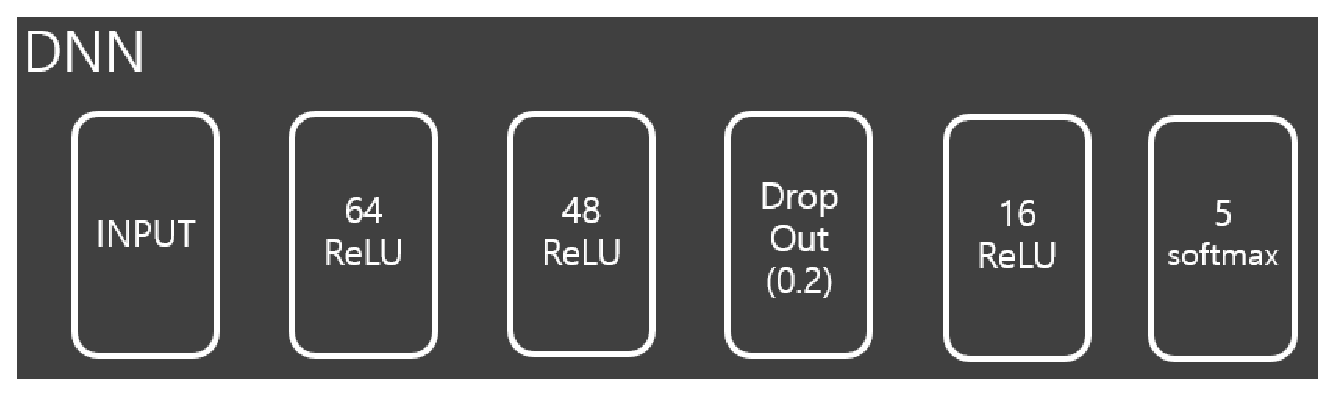
\includegraphics[width=10cm]{DNN.eps}
   \hfil
\caption{Shape of DNN Model}
\label{DNNModel}
\centering
   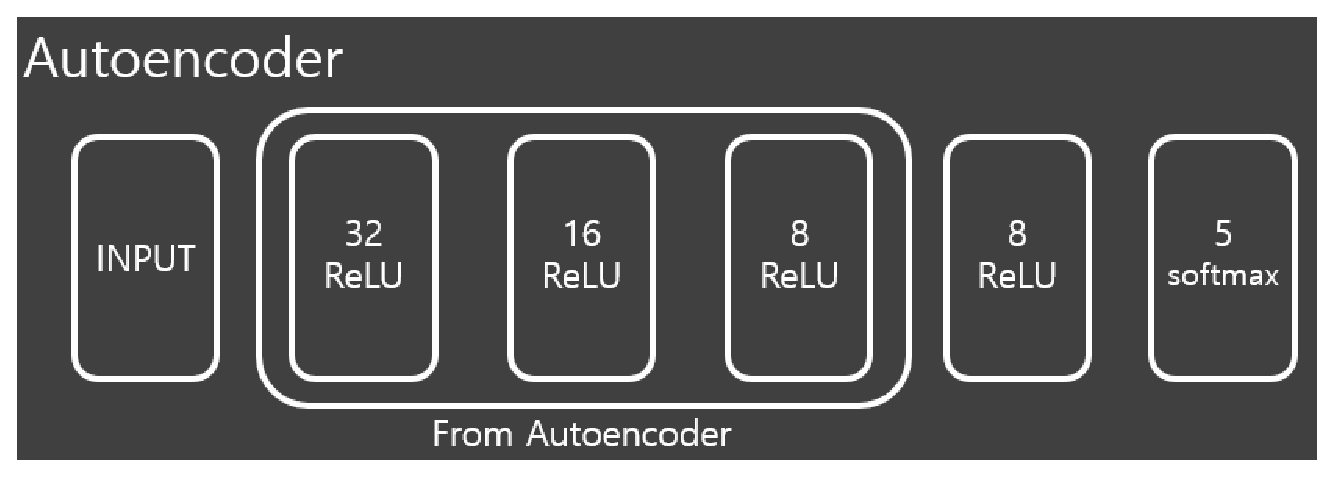
\includegraphics[width=10cm]{Autoencoder.eps}
   \hfil
\caption{Shape of Autoencoder Model}
\label{AutoencoderModel}
\end{figure}


\section{Evaluation}
\label{eval}

Section \ref{eval} discusses the evaluation result of the framework.

\subsection{Environment}
We set up the evaluation environment as follows.
\begin{center}
		\begin{tabular}{|l|r|}
			\multicolumn{2}{c}{\textbf{\large Evaluation Environment}} \\ \hline
			{OS}  & Windows 10  \\ \hline
			{CPU} & AMD Ryzen 3600XT (6C12T)  \\ \hline
			{GPU} & NDIVIA GeForce GTX 1660 SUPER  \\ \hline
			{RAM} & 24GB     \\ \hline
			{Runtime} & Python 3.8 \& Jupyter notebook     \\ \hline
		\end{tabular}
\end{center}

\subsection{Feature set}

The number of all possible feature sets is $2^{41}$, and testing all possible feature sets is almost impossible. So we arbitrary selected five feature set that is considered as meaningful in this project. Below are the feature sets we selected.
\begin{itemize}
    \item [1.] Full feature: Using all extracted features as feature set
    \item [2.] Extended Flow information: All flow information with basic packet information(protocol type, data length)
    \item [3.] Flow information only: Feature set contains only flow information
    \item [4.] Limited flow information: Some flow information([35, 37, 38]) were dropped from above feature set
    \item [5.] Packet information Only:  Feature set with all packet information and without flow information
\end{itemize}

\subsection{Perfomance}
We evalauted the performance of each model with selected feature sets.
\begin{figure}[H]
   \begin{minipage}{0.48\textwidth}
     \centering
           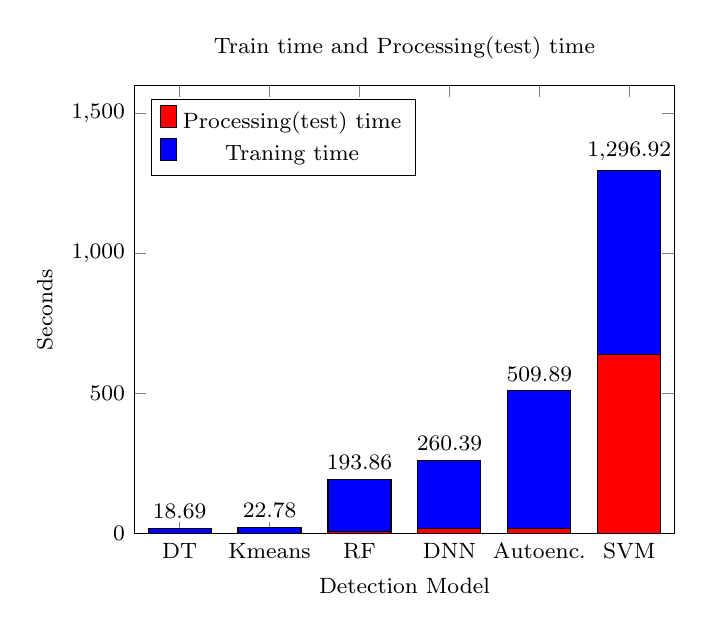
\begin{tikzpicture}
           \tikzstyle{every node}=[font=\footnotesize]
               \pgfplotsset{
                            show sum on top/.style={
                                /pgfplots/scatter/@post marker code/.append code={%
                                    \node[
                                        at={(normalized axis cs:%
                                                \pgfkeysvalueof{/data point/x},%
                                                \pgfkeysvalueof{/data point/y})%
                                        },
                                        anchor=south,
                                    ]
                                    {\pgfmathprintnumber{\pgfkeysvalueof{/data point/y}}};
                                },
                            },
                        }
    
              \begin{axis}[
                title={Train time and Processing(test) time},
                ybar stacked, ymin=0, ymax=1600,
                bar width=8mm,
                symbolic x coords={DT, Kmeans, RF, DNN, Autoenc., SVM},
                xtick=data,
                nodes near coords={},
                xlabel={Detection Model},
                ylabel={Seconds},
                legend pos=north west,
              ]
              \addplot [fill=red] coordinates {
            ({DT},0.283)
            ({Kmeans},0.547)
            ({RF},9.424)
            ({DNN},17.274)
            ({Autoenc.},17.741)
            ({SVM},638.235)};
            \addlegendentry{Processing(test) time}
              \addplot [fill=blue,show sum on top] coordinates {
            ({DT},18.403)
            ({Kmeans},22.237)
            ({RF},184.432)
            ({DNN},243.117)
            ({Autoenc.},492.151)
            ({SVM},658.689)};
            \addlegendentry{Traning time}
            \end{axis}
          \end{tikzpicture}
     \caption{Feature Set \#1}\label{Fig:Data1}
   \end{minipage}\hfill
   \begin{minipage}{0.48\textwidth}
     \centering
     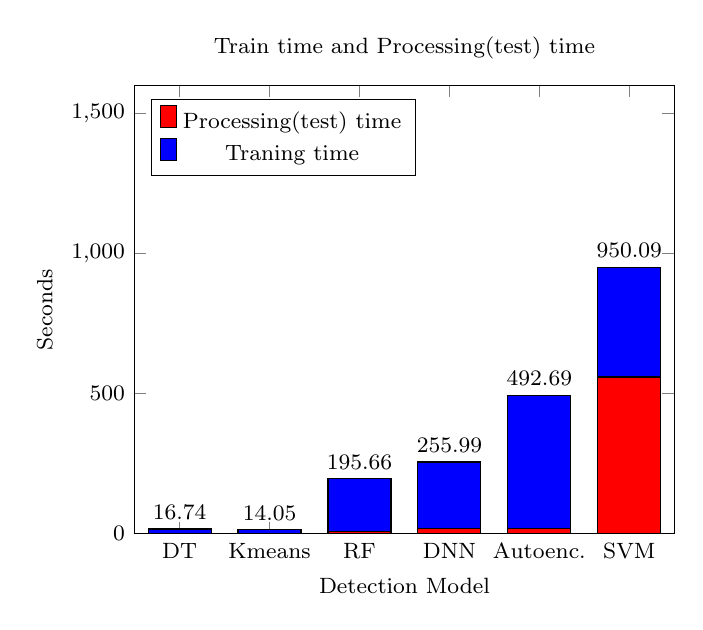
\begin{tikzpicture}
           \tikzstyle{every node}=[font=\footnotesize]
               \pgfplotsset{
                            show sum on top/.style={
                                /pgfplots/scatter/@post marker code/.append code={%
                                    \node[
                                        at={(normalized axis cs:%
                                                \pgfkeysvalueof{/data point/x},%
                                                \pgfkeysvalueof{/data point/y})%
                                        },
                                        anchor=south,
                                    ]
                                    {\pgfmathprintnumber{\pgfkeysvalueof{/data point/y}}};
                                },
                            },
                        }
    
              \begin{axis}[
                title={Train time and Processing(test) time},
                ybar stacked, ymin=0, ymax=1600,
                bar width=8mm,
                symbolic x coords={DT, Kmeans, RF, DNN, Autoenc., SVM},
                xtick=data,
                nodes near coords={},
                xlabel={Detection Model},
                ylabel={Seconds},
                legend pos=north west,
              ]
              \addplot [fill=red] coordinates {
            ({DT},0.196)
            ({Kmeans},0.203)
            ({RF},8.643)
            ({DNN},18.062)
            ({Autoenc.},17.485)
            ({SVM},559.488)};
            \addlegendentry{Processing(test) time}
              \addplot [fill=blue,show sum on top] coordinates {
            ({DT},16.548)
            ({Kmeans},13.850)
            ({RF},187.015)
            ({DNN},237.931)
            ({Autoenc.},475.201)
            ({SVM},390.599)};
            \addlegendentry{Traning time}
            \end{axis}
          \end{tikzpicture}
     \caption{Feature Set \#2}\label{Fig:Data2}
   \end{minipage}
\end{figure}

\begin{figure}[H]
   \begin{minipage}{0.48\textwidth}
     \centering
           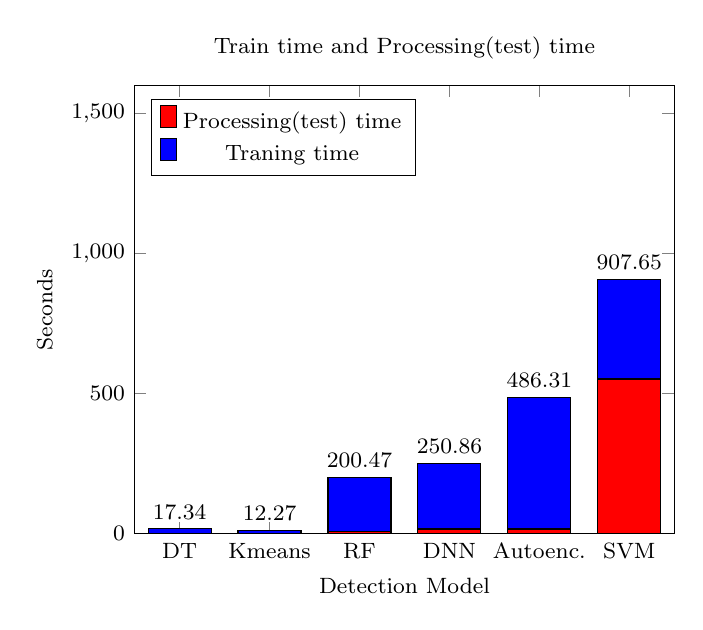
\begin{tikzpicture}
           \tikzstyle{every node}=[font=\footnotesize]
               \pgfplotsset{
                            show sum on top/.style={
                                /pgfplots/scatter/@post marker code/.append code={%
                                    \node[
                                        at={(normalized axis cs:%
                                                \pgfkeysvalueof{/data point/x},%
                                                \pgfkeysvalueof{/data point/y})%
                                        },
                                        anchor=south,
                                    ]
                                    {\pgfmathprintnumber{\pgfkeysvalueof{/data point/y}}};
                                },
                            },
                        }
    
              \begin{axis}[
                title={Train time and Processing(test) time},
                ybar stacked, ymin=0, ymax=1600,
                bar width=8mm,
                symbolic x coords={DT, Kmeans, RF, DNN, Autoenc., SVM},
                xtick=data,
                nodes near coords={},
                xlabel={Detection Model},
                ylabel={Seconds},
                legend pos=north west,
              ]
              \addplot [fill=red] coordinates {
            ({DT},0.202)
            ({Kmeans},0.188)
            ({RF},8.629)
            ({DNN},17.001)
            ({Autoenc.},17.088)
            ({SVM},552.080)};
            \addlegendentry{Processing(test) time}
              \addplot [fill=blue,show sum on top] coordinates {
            ({DT},17.140)
            ({Kmeans},12.082)
            ({RF},191.838)
            ({DNN},233.857)
            ({Autoenc.},469.220)
            ({SVM},355.567)};
            \addlegendentry{Traning time}
            \end{axis}
          \end{tikzpicture}
     \caption{Feature Set \#3}\label{Fig:Data1}
   \end{minipage}\hfill
   \begin{minipage}{0.48\textwidth}
     \centering
     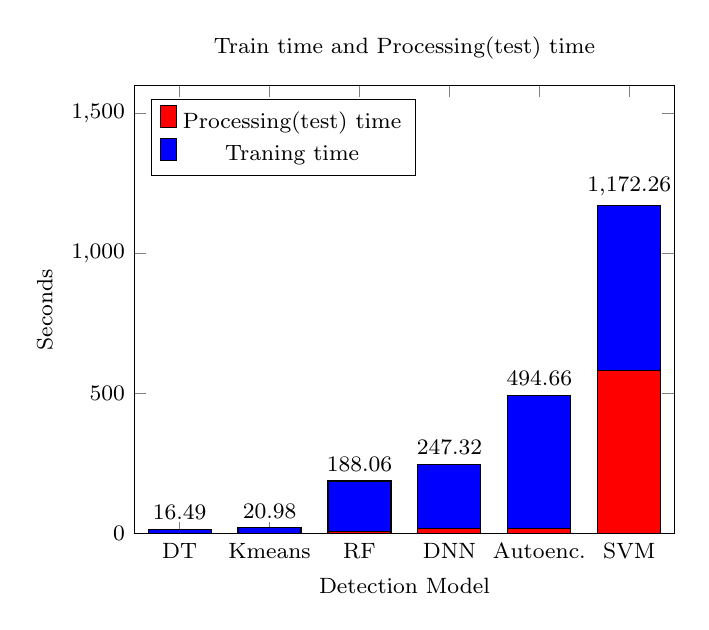
\begin{tikzpicture}
           \tikzstyle{every node}=[font=\footnotesize]
               \pgfplotsset{
                            show sum on top/.style={
                                /pgfplots/scatter/@post marker code/.append code={%
                                    \node[
                                        at={(normalized axis cs:%
                                                \pgfkeysvalueof{/data point/x},%
                                                \pgfkeysvalueof{/data point/y})%
                                        },
                                        anchor=south,
                                    ]
                                    {\pgfmathprintnumber{\pgfkeysvalueof{/data point/y}}};
                                },
                            },
                        }
    
              \begin{axis}[
                title={Train time and Processing(test) time},
                ybar stacked, ymin=0, ymax=1600,
                bar width=8mm,
                symbolic x coords={DT, Kmeans, RF, DNN, Autoenc., SVM},
                xtick=data,
                nodes near coords={},
                xlabel={Detection Model},
                ylabel={Seconds},
                legend pos=north west,
              ]
              \addplot [fill=red] coordinates {
            ({DT},0.283)
            ({Kmeans},0.438)
            ({RF},9.329)
            ({DNN},17.725)
            ({Autoenc.},17.251)
            ({SVM},582.078)};
            \addlegendentry{Processing(test) time}
              \addplot [fill=blue,show sum on top] coordinates {
            ({DT},16.207)
            ({Kmeans},20.540)
            ({RF},178.734)
            ({DNN},229.594)
            ({Autoenc.},477.405)
            ({SVM},590.179)};
            \addlegendentry{Traning time}
            \end{axis}
          \end{tikzpicture}
     \caption{Feature Set \#4}\label{Fig:Data2}
   \end{minipage}
\end{figure}

\begin{figure}[H]
   \begin{minipage}{0.48\textwidth}
     \centering
           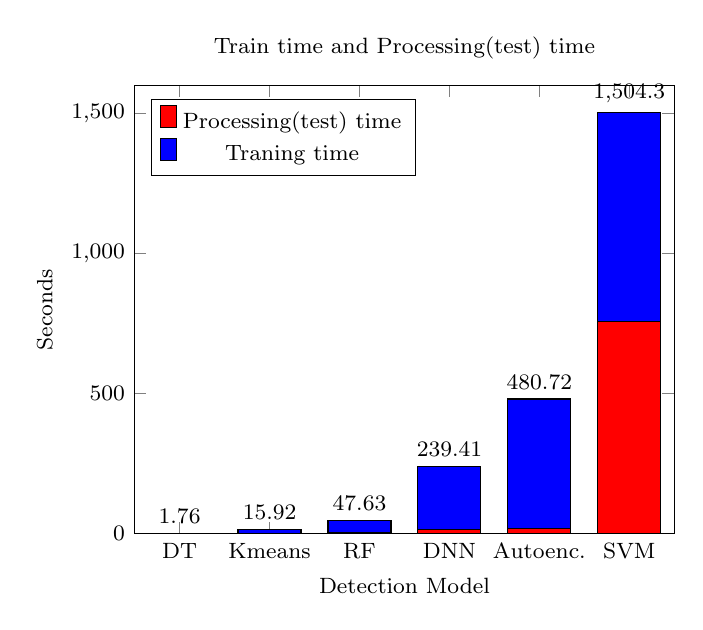
\begin{tikzpicture}
           \tikzstyle{every node}=[font=\footnotesize]
               \pgfplotsset{
                            show sum on top/.style={
                                /pgfplots/scatter/@post marker code/.append code={%
                                    \node[
                                        at={(normalized axis cs:%
                                                \pgfkeysvalueof{/data point/x},%
                                                \pgfkeysvalueof{/data point/y})%
                                        },
                                        anchor=south,
                                    ]
                                    {\pgfmathprintnumber{\pgfkeysvalueof{/data point/y}}};
                                },
                            },
                        }
    
              \begin{axis}[
                title={Train time and Processing(test) time},
                ybar stacked, ymin=0, ymax=1600,
                bar width=8mm,
                symbolic x coords={DT, Kmeans, RF, DNN, Autoenc., SVM},
                xtick=data,
                nodes near coords={},
                xlabel={Detection Model},
                ylabel={Seconds},
                legend pos=north west,
              ]
              \addplot [fill=red] coordinates {
            ({DT},0.172)
            ({Kmeans},0.344)
            ({RF},5.311)
            ({DNN},15.978)
            ({Autoenc.},17.264)
            ({SVM},757.514)};
            \addlegendentry{Processing(test) time}
              \addplot [fill=blue,show sum on top] coordinates {
            ({DT},1.591)
            ({Kmeans},15.575)
            ({RF},42.319)
            ({DNN},223.429)
            ({Autoenc.},463.454)
            ({SVM},746.782)};
            \addlegendentry{Traning time}
            \end{axis}
          \end{tikzpicture}
     \caption{Feature Set \#5}\label{Fig:Data1}
   \end{minipage}\hfill
\end{figure}
Each detection model showed relatively similar performance across the feature sets. To sum up, it is as follows;
\begin{itemize}
    \item In most cases, DT, Kmeans showed the highest performance among detection models in terms of training and test(process) time.
    \item DNN, Autoencoder, Random Forest models showed the second-fastest performance. They spent more training times, but they showed fast detection speed in comparison with DT and Kmeans model
    \item SVM showed low performance in most cases, including both training time and test time.
    \item Reducing the number of features in feature set reduced training time and test time of some model, such as SVM.
\end{itemize}

\subsection{Accuracy}
We evaluated the performance of each model with selected feature sets.

\begin{figure}[H]
   \begin{minipage}{0.48\textwidth}
     \centering
           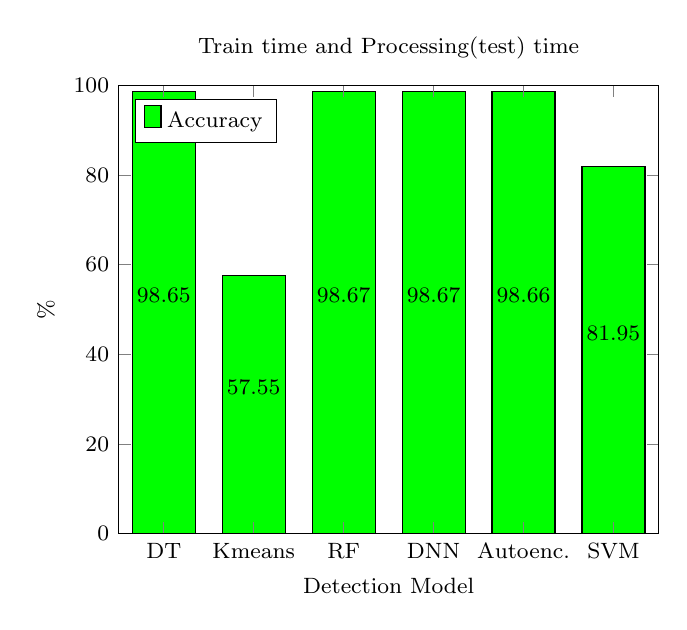
\begin{tikzpicture}
           \tikzstyle{every node}=[font=\footnotesize]
              \begin{axis}[
                title={Train time and Processing(test) time},
                ybar stacked, ymin=0, ymax=100,
                bar width=8mm,
                symbolic x coords={DT, Kmeans, RF, DNN, Autoenc., SVM},
                xtick=data,
                nodes near coords,
                nodes near coords align={vertical},
                xlabel={Detection Model},
                ylabel={\%},
                legend pos=north west,
                axis on top,
              ]
              \addplot [fill=green] coordinates {
            ({DT},98.653)
            ({Kmeans},57.550)
            ({RF},98.667)
            ({DNN},98.671)
            ({Autoenc.},98.663)
            ({SVM},81.950)};
            \addlegendentry{Accuracy}
            \end{axis}
          \end{tikzpicture}
     \caption{Feature Set \#1}\label{Fig:Data1}
   \end{minipage}\hfill
   \begin{minipage}{0.48\textwidth}
     \centering
     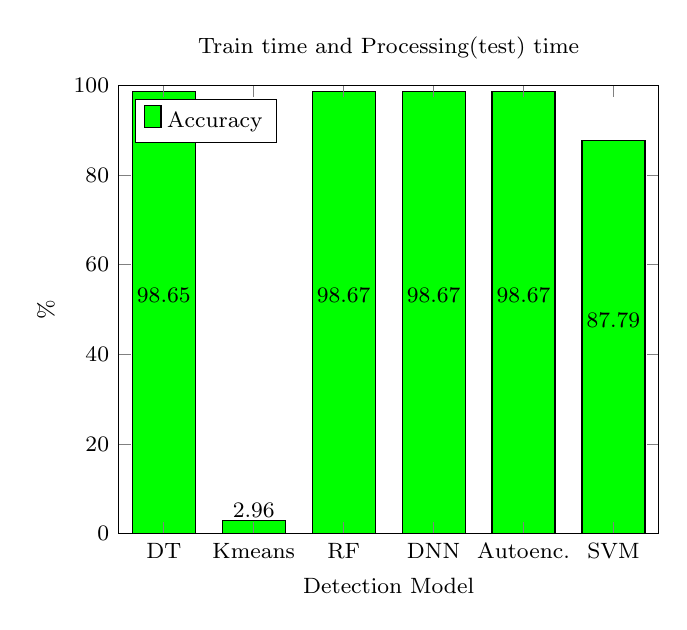
\begin{tikzpicture}
           \tikzstyle{every node}=[font=\footnotesize]
              \begin{axis}[
                title={Train time and Processing(test) time},
                ybar stacked, ymin=0, ymax=100,
                bar width=8mm,
                symbolic x coords={DT, Kmeans, RF, DNN, Autoenc., SVM},
                xtick=data,
                nodes near coords,
                nodes near coords align={vertical},
                xlabel={Detection Model},
                ylabel={\%},
                legend pos=north west,
                axis on top,
              ]
              \addplot [fill=green] coordinates {
            ({DT},98.653)
            ({Kmeans},2.956)
            ({RF},98.668)
            ({DNN},98.669)
            ({Autoenc.},98.673)
            ({SVM},87.789)};
            \addlegendentry{Accuracy}
            \end{axis}
          \end{tikzpicture}
     \caption{Feature Set \#2}\label{Fig:Data2}
   \end{minipage}
\end{figure}

\begin{figure}[H]
   \begin{minipage}{0.48\textwidth}
     \centering
           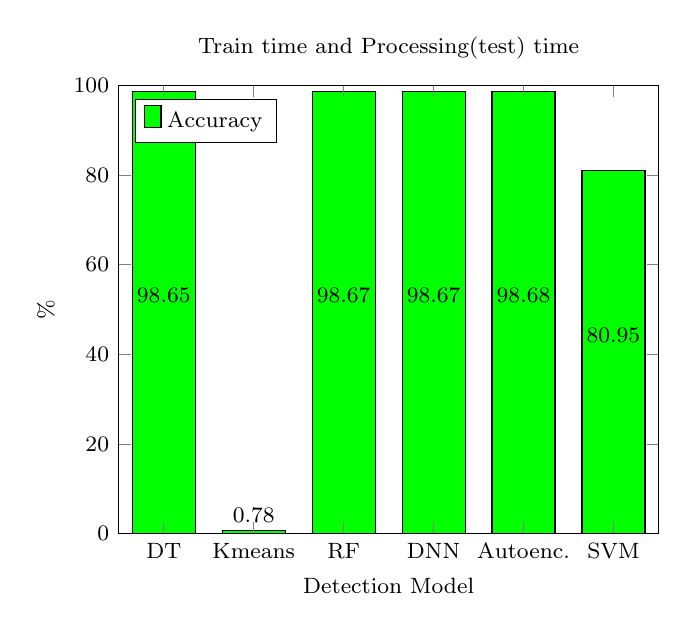
\begin{tikzpicture}
           \tikzstyle{every node}=[font=\footnotesize]
              \begin{axis}[
                title={Train time and Processing(test) time},
                ybar stacked, ymin=0, ymax=100,
                bar width=8mm,
                symbolic x coords={DT, Kmeans, RF, DNN, Autoenc., SVM},
                xtick=data,
                nodes near coords,
                nodes near coords align={vertical},
                xlabel={Detection Model},
                ylabel={\%},
                legend pos=north west,
                axis on top,
              ]
              \addplot [fill=green] coordinates {
            ({DT},98.652)
            ({Kmeans},0.779)
            ({RF},98.668)
            ({DNN},98.667)
            ({Autoenc.},98.675)
            ({SVM},80.948)};
            \addlegendentry{Accuracy}
            \end{axis}
          \end{tikzpicture}
     \caption{Feature Set \#3}\label{Fig:Data1}
   \end{minipage}\hfill
   \begin{minipage}{0.48\textwidth}
     \centering
     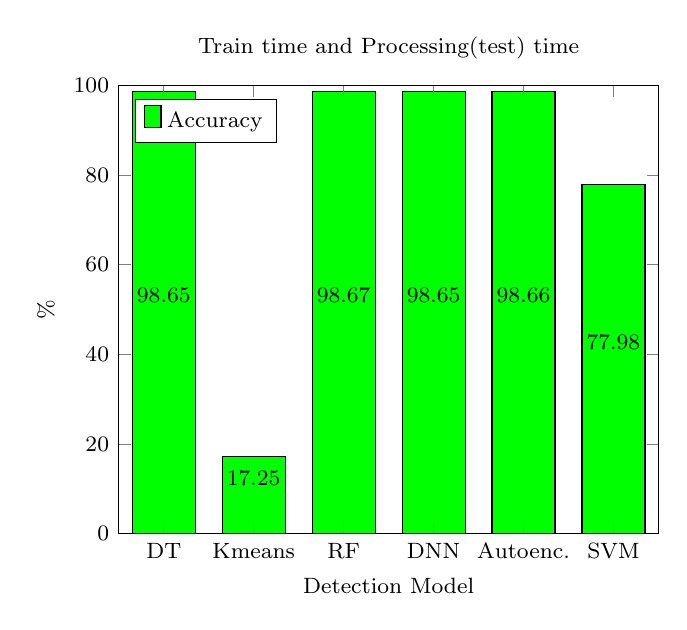
\begin{tikzpicture}
           \tikzstyle{every node}=[font=\footnotesize]
              \begin{axis}[
                title={Train time and Processing(test) time},
                ybar stacked, ymin=0, ymax=100,
                bar width=8mm,
                symbolic x coords={DT, Kmeans, RF, DNN, Autoenc., SVM},
                xtick=data,
                nodes near coords,
                nodes near coords align={vertical},
                xlabel={Detection Model},
                ylabel={\%},
                legend pos=north west,
                axis on top,
              ]
              \addplot [fill=green] coordinates {
            ({DT},98.651)
            ({Kmeans},17.248)
            ({RF},98.670)
            ({DNN},98.654)
            ({Autoenc.},98.658)
            ({SVM},77.975)};
            \addlegendentry{Accuracy}
            \end{axis}
          \end{tikzpicture}
     \caption{Feature Set \#4}\label{Fig:Data2}
   \end{minipage}
\end{figure}

\begin{figure}[H]
   \begin{minipage}{0.48\textwidth}
     \centering
           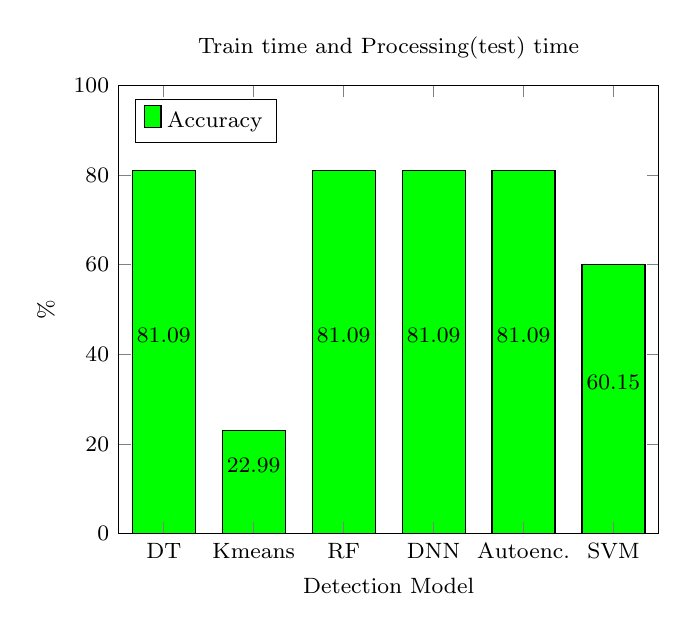
\begin{tikzpicture}
           \tikzstyle{every node}=[font=\footnotesize]
              \begin{axis}[
                title={Train time and Processing(test) time},
                ybar stacked, ymin=0, ymax=100,
                bar width=8mm,
                symbolic x coords={DT, Kmeans, RF, DNN, Autoenc., SVM},
                xtick=data,
                nodes near coords,
                nodes near coords align={vertical},
                xlabel={Detection Model},
                ylabel={\%},
                legend pos=north west,
                axis on top,
              ]
              \addplot [fill=green] coordinates {
            ({DT},81.093)
            ({Kmeans},22.987)
            ({RF},81.093)
            ({DNN},81.091)
            ({Autoenc.},81.091)
            ({SVM},60.150)};
            \addlegendentry{Accuracy}
            \end{axis}
          \end{tikzpicture}
     \caption{Feature Set \#5}\label{Fig:Data1}
   \end{minipage}\hfill
\end{figure}

Each detection model showed relatively similar performance across the feature sets. To sum up, it is as follows;
\begin{itemize}
    \item In most cases, feature sets containing flow information showed high accuracy across detection models. It is, even if the accuracy of a specific detection model is low on average, the model with a feature set including flow information showed higher accuracy than one without flow information relatively.
    \item DT, DNN, Autoencoder, Random Forest showed the highest accuracy among detection models in terms of detection accuracy.
    \item SVM showed the second accurate result. But accuracy difference between the above models is big.
    \item Kmeans model was inaccurate than others, lower than 50\% in most cases. It showed a weak correlation between feature selection and accuracy.
\end{itemize}

\subsection{Evaluation Summary}
From the evaluation of the feature set and detection model, we could reach some conclusions.
\begin{itemize}
    \item Flow information is more efficient than packet information when detecting Modbus/TCP anomaly. Detecting anomaly with packet information of each packet also works, but the accuracy of only using flow information is almost the same as using all features. \item Removing some part of feature increase performance slightly but reduces accuracy in a trade-off. 
    \item In this project, DT was the best model in terms of performance accuracy. We guess that it is because attack types in the dataset are simple or DT is indeed a good model to detect an anomaly. 
    \item DNN, Random Forest, and autoencoder model also showed an acceptable level of performance and high accuracy. 
    \item Other two models are not recommended to be used. SVM shows less accuracy and worse performance than other models, and Kmeans model failed to detect anomalies properly.
\end{itemize}

\section{Future Work}
\label{future}
Section \ref{future} discusses the limitation of the project and future research topics.

\subsection{Collecting Dataset and Detection Model}
In this project, we used a packet third-party dataset available since we do not have access to the real-world or simulated industrial network. The dataset used in this project is well-generated, but attack types are not varied enough. Collecting more datasets is required for these reasons.
\begin{itemize}
    \item[] Coverage: models have to detect various attack types/scenarios.
    \item[] Validation: accuracy of the trained model have to be robust against multiple datasets in detecting an anomaly.
\end{itemize}
Therefore, collecting available datasets with more attack types/scenarios and generating dataset by ourself can be one of the future work. Also, recently devised learning-based models need to be applied to the framework. Including the latest learning-based models into our framework also should be considered as future work.  

\subsection{Feature Analysis} 
Because of lack of time, we did not analyze exactly which feature is helpful to detect exactly which attack type. It should be done because we can reduce features of a feature set that are not useful to detect any anomaly attack. Analyzing the relation between each feature and accuracy of detecting specific attack type/scenario.

\section{Conclusion}
We proposed the framework for evaluating feature set and learning-based models to efficiently and accurately detect Modbus/TCP anomalies. We evaluated five different feature sets with various learning-based models. Among feature sets and models, feature sets containing the information about packet flow showed high accuracy, and DT, DNN, Random Forest, and Autoencoder models showed high performance and accuracy enough to be applied in the real world. We expect the project result can help design the ICS anomaly detection model in the future.

\bibliography{ref}
\bibliographystyle{acm}


\end{document}
 